\let\negmedspace\undefined
\let\negthickspace\undefined
\documentclass[journal]{IEEEtran}
\usepackage[a5paper, margin=10mm, onecolumn]{geometry}
\usepackage{tfrupee}

\setlength{\headheight}{1cm}
\setlength{\headsep}{0mm}

\usepackage{gvv-book}
\usepackage{gvv}
\usepackage{cite}
\usepackage{amsmath,amssymb,amsfonts,amsthm}
\usepackage{algorithmic}
\usepackage{graphicx}
\usepackage{textcomp}
\usepackage{xcolor}
\usepackage{txfonts}
\usepackage{listings}
\usepackage{enumitem}
\usepackage{mathtools}
\usepackage{gensymb}
\usepackage{comment}
\usepackage[breaklinks=true]{hyperref}
\usepackage{tkz-euclide} 
\usepackage{listings}
\def\inputGnumericTable{}                            
\usepackage[latin1]{inputenc}                            
\usepackage{color}                                  
\usepackage{array}                                  
\usepackage{longtable}                               
\usepackage{calc}                                   
\usepackage{multirow}                               
\usepackage{hhline}                                 
\usepackage{ifthen}                                 
\usepackage{lscape}
\usepackage{float}  % <-- Add this to allow [H] in figures

\begin{document}


\bibliographystyle{IEEEtran}

\title{2.7.15}
\author{EE25BTECH11003 - Adharvan Kshathriya Bommagani}
\maketitle


\renewcommand{\thefigure}{\theenumi}
\renewcommand{\thetable}{\theenumi}
\setlength{\intextsep}{10pt} % Space between text and floats
\textbf{Question}:\\
Find the volume of a parallelepiped whose edges are given by $-3\hat{i} + 7\hat{j} + 5\hat{k}$, $-5\hat{i} + 7\hat{j} - 3\hat{k}$ and $7\hat{i} - 5\hat{j} - 3\hat{k}$.\\
  


\textbf{Solution:}
Let $\vec{a}$, $\vec{b}$ and $\vec{c}$ be the vectors representing the edges of the parallelepiped.
\begin{align}
\vec{a} &= \myvec{-3 \\ 7 \\ 5}, \quad 
\vec{b} = \myvec{-5 \\ 7 \\ -3}, \quad 
\vec{c} = \myvec{7 \\ -5 \\ -3}
\end{align}



The volume of the parallelepiped is given by the absolute value of the scalar triple product:
\begin{align*}
V = \left| \left[ \vec{a} \ \vec{b} \ \vec{c} \right] \right|
\end{align*}

which is equivalent to the determinant of the matrix formed by the components of $\vec{a}$, $\vec{b}$, and $\vec{c}$:
\begin{align*}
V = \left| \myvec{ -3 & -5 & 7 \\ 7 & 7 & -5 \\ 5 & -3 & -3 } \right|
\end{align*}



The determinant expression:
\begin{align*}
\det = -3(-36) + 5(4) + 7(-56) = 108 + 20 - 392 = -264
\end{align*}

Thus, the volume is:
\begin{align*}
V = \left| -264 \right| = 264 \text{ cubic units}
\end{align*}

Therefore, the volume of the parallelepiped is 264 cubic units.

\newpage
\textbf{Parellelopiped Defined by Vectors a, b and c:}
\begin{figure}[h]
    \centering
    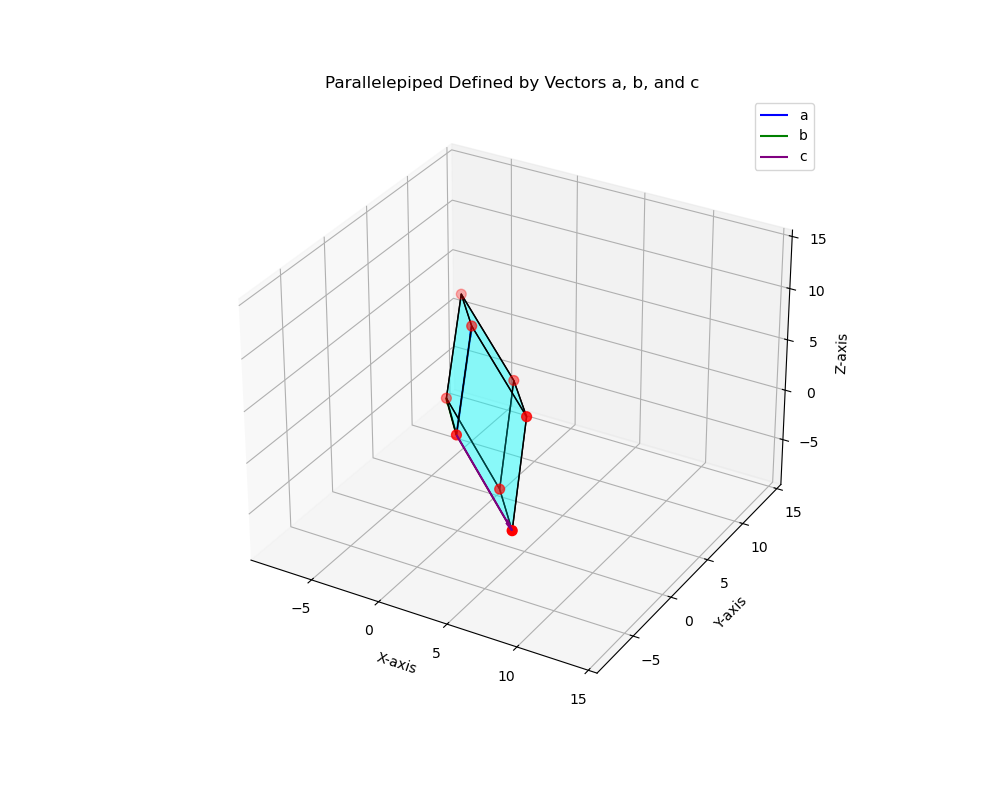
\includegraphics[width=1.1\columnwidth]{figs/fig1.png}
    \caption{Figure for 2.7.15}
    \label{fig1}
\end{figure}

\end{document}
